\documentclass{article}

% if you need to pass options to natbib, use, e.g.:
%     \PassOptionsToPackage{numbers, compress}{natbib}
% before loading neurips_2018

% ready for submission
% \usepackage{neurips_2018}

% to compile a preprint version, e.g., for submission to arXiv, add add the
% [preprint] option:
%     \usepackage[preprint]{neurips_2018}

% to compile a camera-ready version, add the [final] option, e.g.:
     \usepackage[final]{neurips_2018}

% to avoid loading the natbib package, add option nonatbib:
%     \usepackage[nonatbib]{neurips_2018}

\usepackage[utf8]{inputenc} % allow utf-8 input
\usepackage[T1]{fontenc}    % use 8-bit T1 fonts
\usepackage{hyperref}       % hyperlinks
\usepackage{url}            % simple URL typesetting
\usepackage{booktabs}       % professional-quality tables
\usepackage{amsfonts}       % blackboard math symbols
\usepackage{nicefrac}       % compact symbols for 1/2, etc.
\usepackage{microtype}      % microtypography
\usepackage{graphicx}

\title{MINST Kaggle Digit Recognizer: Contrasting the Random Forest and MLP Neural Network}

% The \author macro works with any number of authors. There are two commands
% used to separate the names and addresses of multiple authors: \And and \AND.
%
% Using \And between authors leaves it to LaTeX to determine where to break the
% lines. Using \AND forces a line break at that point. So, if LaTeX puts 3 of 4
% authors names on the first line, and the last on the second line, try using
% \AND instead of \And before the third author name.

\author{%
   Andrew Osborne \\
   \texttt{amo004@uark.edu} \\
   \And
   Josh Price \\
   \texttt{jdp024@uark.edu} \\
   \AND
   April Walker \\
   \texttt{adw027@uark.edu} \\
   \\
   University of Arkansas, \\
   Fayetteville, AR, 72701, USA
}

\begin{document}
% \nipsfinalcopy is no longer used

\maketitle

\begin{abstract}
  In order to tackle the classic MINST dataset, our team implemented a random forest (RF) and a multi-layer perception (MLP) classifier using the \verb+sklearn+ Python library. As expected from a high-dimensional problem such as digit recognition, our RF preformed sub-optimally. Contrasting the accuracy between our training data and testing data suggest severe overfitting. Our final Kaggle submission reached a correct prediction rate of 96.66\%. In order to optimize our MLP NN, we explored the use of stochastic and Adam gradient descent, however found the later consistently outperformed the former. In order to balance accuracy vs. complexity, our cross validation method suggests the use of 1 hidden layer and 512 nodes. Our final Kaggle submission resulted in a correct prediction rate of 97.90\%, suggesting our NN is well-trained. While our MLP preformed considerably better than our RF, the training took approximately 60 times as long, implying the RF may be a desirable option when speed is of utmost importance. 
\end{abstract}

\section{The MINST Dataset}
The MNIST digit database is a classic starting point for individuals wanting to learn the basics of computer vision and get hands on experience with machine learning algorithms. The dataset is composed of 70,000 28x28 pixel grey-scale images of handwritten numbers between zero and nine [6]. The pre-flattened Kaggle dataset provides you with 42,000 training examples and 28,000 testing examples. Each 28x28 pixel image is represented by a 784 length vector with each element containing some integer between 0 and 255 representing the lightness or darkness of that pixel. Additionally, the training dataset provides the correct labels for each image. These images can be reshaped and rendered from the provided dataset as shown in Figure 1. 
\begin{figure}[h]
  \centering
    \begin{minipage}[t]{0.3\textwidth}
        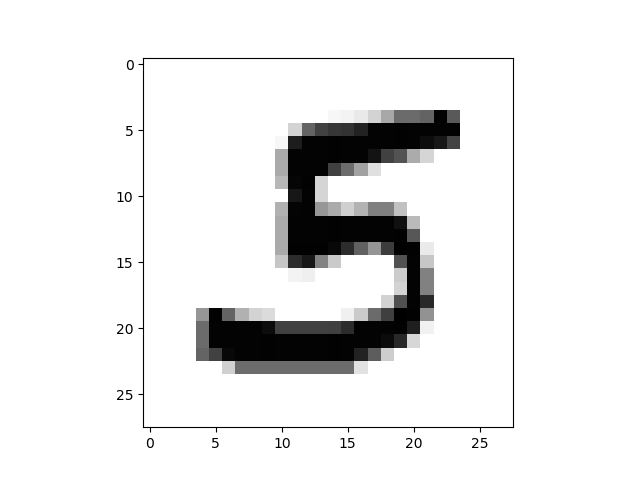
\includegraphics[width=\textwidth]{img786render.png}
    \end{minipage}
    \begin{minipage}[t]{0.3\textwidth}
        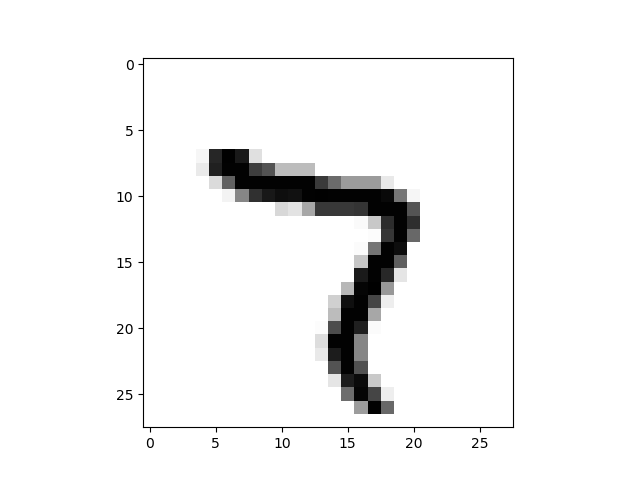
\includegraphics[width=\textwidth]{img98render.png}
    \end{minipage}
    \begin{minipage}[t]{0.3\textwidth}
        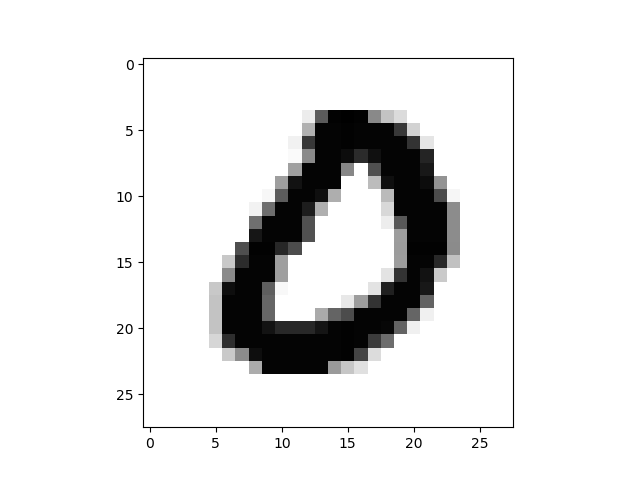
\includegraphics[width=\textwidth]{img6render.png}
    \end{minipage}
  \caption{Image Renderings from the MNIST Dataset}
\end{figure}
\section{GridSearchCV}
For both machine learning algorithms, training and cross-validation was done using \verb+sklearn+'s \verb+model_selection.GridSearchCV+. The grid search takes in a grid of the hyper-parameters the user wishes to contrast and exhaustively considers all possible parameter combinations. Rather than train the data on the entire training dataset, \verb+GridSearchCV+ partitions the data into $k$ sections then trains the data on $k-1$ of the sections, leaving the last partition as a pseudo-test dataset. The mean cross-validation score (CVS) is the averaged prediction rate over all $k$ segments of the training data, and the hyper-parameter combination with the best mean CVS is chosen [4]. 

\section{Random Forest}
A Random Forest (RF) is a common starting algorithm for those new to machine learning. This is in part due to it's easy of use, but also due to it's flexibility. While in this assignment it is used for classification, it can be also be used in regression problems [2]. Each tree is formed from a bootstrap sample (random sampling with replacement) then grown very similarly to a decision tree. Rather than searching for the very best split feature, it chooses the best of a random subset.\verb+Sklearn+'s \verb+RandomForestClassifier+ combines the probabilistic prediction of each tree, as this has been shown to preform better than the traditional approach of picking a classification based on a majority vote [4,5].

These models are generally very fast to train, but depending on the complexity, can suffer from slow run-time performance. Generally speaking, overfitting can be negated by simple adding more trees to your model [2]. This approach eventually results in diminishing returns, and for high-dimensional problems such as digit recognition, is especially impractical [5].

\subsection{Implementation}
The 784 length vector of input data is normalized to range from 0 to 1 using \verb+sklearn+'s \verb+preprocessing.minmax_scale+. In order to improve our model's predictive power, we contrasted the results from our hyper-parameters \verb+n_estimators+ (number of trees) and  \verb+min_samples_split+ (minimum number of leafs required to split a node). Specifically we allowed 10, 50, 100, and 300 trees to be developed and 2, 4, 8, and 16 as the minimum number of leafs. The later can be thought of as a measure of complexity, with lower minimum resulting in higher complexity. Once the code was prepared, training took approximately 45 seconds. 
\begin{figure}[h]
    \centering
    \begin{minipage}[t]{0.45\textwidth}
        \centering
        \textbf{(A)}
        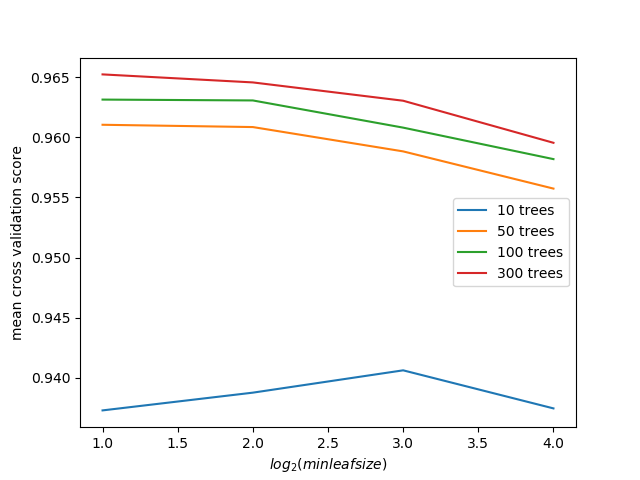
\includegraphics[width=\textwidth]{CVscoreVsLeafSize.png}
    \end{minipage}
    \begin{minipage}[t]{0.45\textwidth}
        \centering
        \textbf{(B)}
        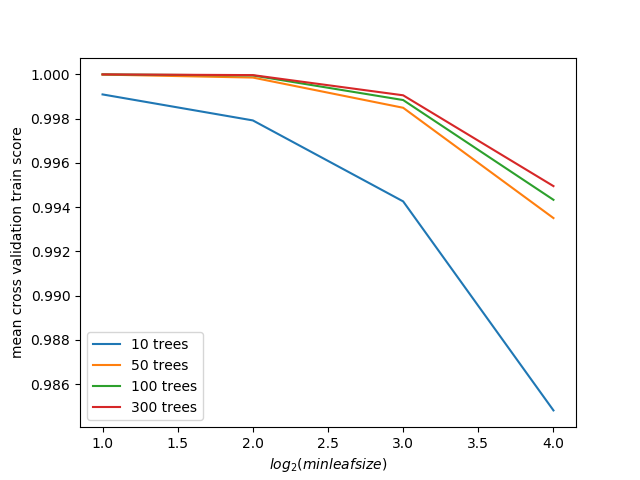
\includegraphics[width=\textwidth]{CVtestVsLeafSize.png}
    \end{minipage}
\caption{(A,B) Cross Validation of Hyper-parameters for (A) training data and (B) testing data by contrasting mean cross validation score and $\log_2(minleafsize)$ giving the minimum leaf threshold as a measure of complexity. The scores for varying numbers of trees are shown.}
\end{figure}

\subsection{Cross-Validation and Results}
Training and cross-validation was done using \verb+model_selection.GridSearchCV+. In order to visualize the results, Figure 2 contrasts the mean CVS and prediction rates of the training and test datasets. The $\log_2(minleafsize)$ which inversely measures the complexity suggests the more complex models preform outstandingly against the training data but have little impact on the testing data. Adding trees has a similar positive affect on both datasets, however, also decreases exponentially as more trees are added. These results suggest that our model suffers from extreme levels of overfitting. As expected, adding trees does improve our models predictive power but isn't the most practical for our dataset. Our Kaggle submission of 300 trees and a minimum leaf number of 2 gave a prediction rate of 96.6\%

\section{Multi-Layer Perceptron Classifier}
A Multi-layer Perceptron (MLP) is a type of deep neural network (NN) that is trained using backpropogation. An MLP consists of at least one hidden layer (HL), an input (features) layer, and an output (targets) layer [2].  

\subsection{Contrasting Gradient Descent Algorithms}
A key component of implementing any model using backpropogation is choosing an appropriate gradient descent (GD) algorithm. For our MLP, we decided to contrast stochastic gradient descent (SGD) and Adaptive Moment Estimation (Adam) gradient descent developed by Kingma and Lei Ba [3]. As we've discussed in class, stochastic gradient descent approximates the gradient by considering a single training example at a time. Adam gradient descent is actually an optimized SGD which computes adaptive learning rates for each parameter. This method stores exponentially decaying averages of the past gradient $\nabla_\theta f_t(\theta_{t-1})$ and square of the gradient $\nabla_\theta f_t(\theta_{t-1})^2$ as estimates of the first and second moment of the gradient (mean $m_t$ and variance $v_t$ respectively). The exponential decay rates $\beta_1$ and $\beta_2$ are initialized (generally near 1)\footnote{The developers recommended default is $\beta_1 = 0.9$ and $\beta_2 = 0.999$. [3]} such that the moments can be more specifically calculated using the following:
$$m_t \leftarrow \beta_1 \cdot m_{t-1} + (1-\beta_1)\cdot \nabla_\theta f_t(\theta_{t-1}) $$
$$v_t \leftarrow \beta_2 \cdot v_{t-1} + (1-\beta_2)\cdot \nabla_\theta f_t(\theta_{t-1})^2 $$
With the initial $m_0$ and $v_0$ set to 0. In order to correct for bias, the following bias-corrected moments are then computed:
$$\hat{m_t} \leftarrow m_t/(1-\beta_1^t)$$
$$\hat{v_t} \leftarrow v_t/(1-\beta_2^t)$$
With $\beta_1^t$ and $\beta_2^t$ indicating $\beta_1$ and $\beta_2$ to the power of $t$. Given some $\alpha$ and $\epsilon$ as regularization parameters, the parameters $\theta_t$ are then updated using the following:
$$\theta_t \leftarrow \theta_{t-1} - \alpha \cdot \hat{m_t}/(\sqrt{\hat{v_t}+\epsilon})$$
This process is repeated until $\theta$ converges [3].   

\subsection{Implementation}
In addition to contrasting GD algorithms, the number of hidden nodes were varied between 128, 256, and 512; the number of hidden layers were either 1 or 2; the regularization term $\alpha$ was varied at 0.5, 0.1, 0.001, and 0.0001. The other regularization parameter's for Adam GD were kept at the developer's (Kingma and Lei Ba) recommended defaults: $\epsilon = 10^{-8}$, $\beta_1=0.9$, and $\beta_2=0.999$ [3]. While the learning rate was not varied, an adaptive rate was chosen which divides the current learning rate by 5 with a starting value of $0.001$ [4]. One the code was prepared, training took approximately 46 minutes.

\subsection{Cross-Validation and Results}
Training and cross-validation was done using \verb+model_selection.GridSearchCV+. In order to visualize the results, Figure 2 contrasts the mean CVS and prediction rates of the training and test datasets. A measure of complexity is given by $-log_{10}$ meaning lower $\alpha$ values correspond to higher complexity. As expected, Adam gradient descent was the clear winner across the board. Note that the smaller $\alpa$ value (that is the larger $-\log_{10}(\alpha)$ value) almost consistently improves the prediction rate in (A), but for (B) in some cases causes severe prediction penalties. Examples most obvious example of this is at 1 HL and 256 nodes in (B). Our "winning" model with 1 HL and 512 nodes preformed rather consistently between training and testing datasets. The Kaggle submission of this model gave a prediction rate of 97.90\%.

\begin{figure}[h]
    \centering
    \begin{minipage}[t]{0.45\textwidth}
        \centering
        \textbf{(A)}
        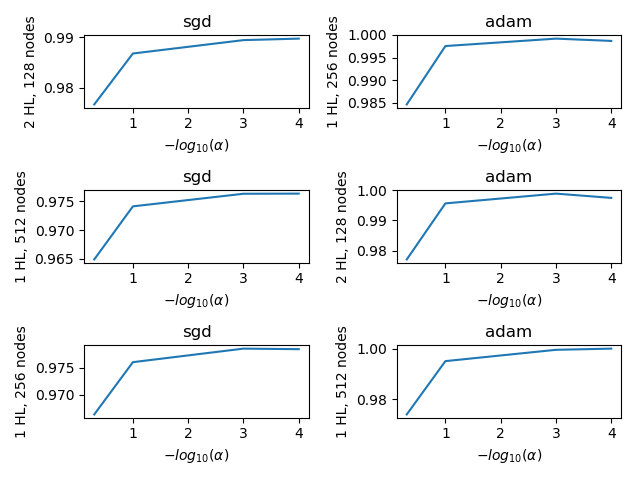
\includegraphics[width=\textwidth]{TrainscoreVsAlpha.png}
    \end{minipage}
    \begin{minipage}[t]{0.45\textwidth}
        \centering
        \textbf{(B)}
        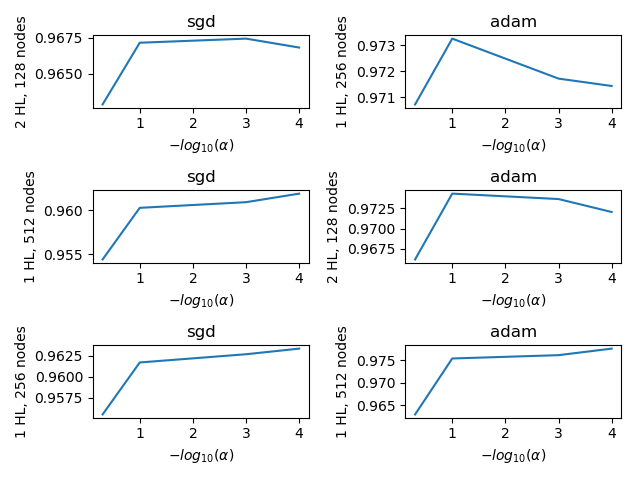
\includegraphics[width=\textwidth]{CVscoreVsAlpha.png}
    \end{minipage}
\caption{(A,B) Cross Validation of Hyper-parameters for (A) training data and (B) testing data by contrasting the mean CVS in (A) and the prediction accuracy in (B) with $-\log_{10}(\alpha)$ giving a measure of complexity. For both (A) and (B), the left colomn gives the results for SGD, and the right colmn gives the results for Adam GD.}
\end{figure}

\section{Conclusions}
As expected, our MLP was better suited for handwritten digit recognition. It is possible that data processing to reduce dimensional would help the RF preform better, however computer vision problems are still better left in the hands of NN's and similar models. One advantage of the RF is it's training time was approximately $1/60^{th}$ of our MLP's, however adding addition trees would begin to bridge this gap and further reduce it's run time speed. 

\clearpage

\section*{References}
\medskip

\small

[1] Bernard, S., Adam, S., & Heutte, L. (2007). \textit{Using Random Forests for Handwritten Digit Recognition}. Ninth International Conference on Document Analysis and Recognition (ICDAR 2007) Vol 2. doi:10.1109/icdar.2007.4377074

[2] Hastie, T., Tibshirani, R., & Friedman, J. H. (2017). The Elements of Statistical Learning: Data Mining, Inference, and Prediction. New York, NY: Springer.

[3] Kingma, D. P., & Lei Ba, J. (2015). 
\textit{Adam: A Method for Stochastic Optimization}. Conference Paper at ICLR. Retrieved from https://arxiv.org/abs/1412.6980.

[4] Pedregosa \textit{et al} (2011) \textit{Scikit-learn: Machine Learning in Python}. JMLR 12, pp. 2825-2830.

[5] Robnik-Šikonja, M. (2004). \textit{Improving Random Forests.} Machine Learning: ECML 2004 Proceedings, Springer, Berlin, 359-370.

[6] Y. LeCun \textit{et al} (1995) \textit{Learning Algorithms For Classification: A Comparison On Handwritten Digit Recognition}, in Oh, J. H. and Kwon, C. and Cho, S. (Eds), Neural Networks: The Statistical Mechanics Perspective, 261-276, World Scientific.

\end{document}
